\documentclass[a4paper,10pt]{article}
%\usepackage[utf8x]{inputenc}

\usepackage{graphicx}
\usepackage{float}
\usepackage{caption}
\usepackage{subcaption}

\usepackage{amsmath}

\title{Assignment 3: Image Alignment and Stitching}
\author{Taco Cohen \& Robrecht Jurriaans\\ (6394590) \& (5887380)}

\begin{document}

\maketitle

\section{Image Alignment}

To align two images, we use the standard procedure:
\begin{enumerate}
 \item Find keypoints in both images
 \item Compute descriptors for each keypoint
 \item Compute matches between keypoints
 \item Estimate the Affine transformation using RANSAC
\end{enumerate}

In the previous assignment we have looked at keypoint detection, descriptors and matching.
As requested in the current assignment, we have used the \verb+vl_feat+ SIFT implementation for these three stages.
This procedure is straightforward, and can be found in \verb+imageAlign.m+, where we use \verb+vl_sift+ to detect and describe keypoints,
and \verb+vl_ubcmatch+ to do the matching.
The result is a set of point correspondences, which we pass to our \verb+ransacA.m+ function, where we perform robust fitting of an affine transformation.

Next, we perform RANSAC with an affine transformation model.
An affine transformation in 2D has $6$ parameters, and since each 2D-point correspondence gives us two equations, we need 3 point correspondences.
We simply perform the RANSAC algorithm as described in the excercise, and to estimate the transformation we use a simple linear least squares (using the pseudo inverse, as described in the assignment).

To see the result, simply run \verb+AlignmentDemo.m+, or see figure \ref{fig:matches} and \ref{fig:transformedA}.
The first image that is plotted shows the two images with the keypoints from the left image, and the corresponding transformed keypoints in the right image (with corresponding points linked by a line).
Note that the keypoints in the right image are \emph{not} the keypoints found in that image.
The second image that is plotted shows the two images, and the transformation of image one to image two, and vice versa.

\begin{figure}
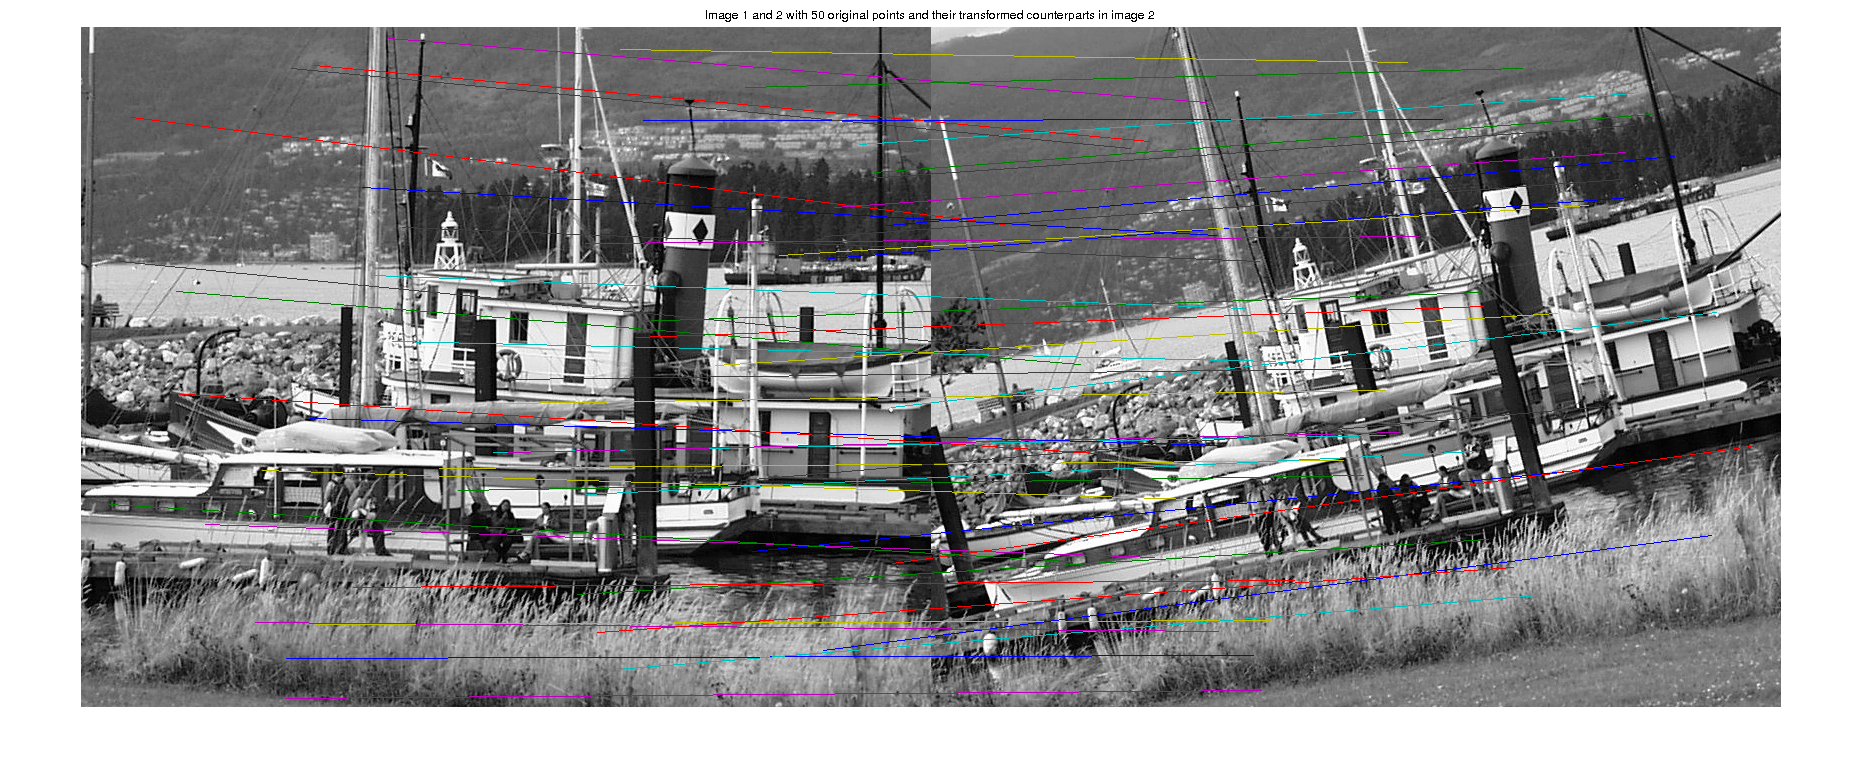
\includegraphics[width=1\textwidth]{img/matchingpoints}
\caption{Keypoints in the left image, and the same points transformed, plotted over the right image.}
\label{fig:matches}
\end{figure}

\begin{figure}
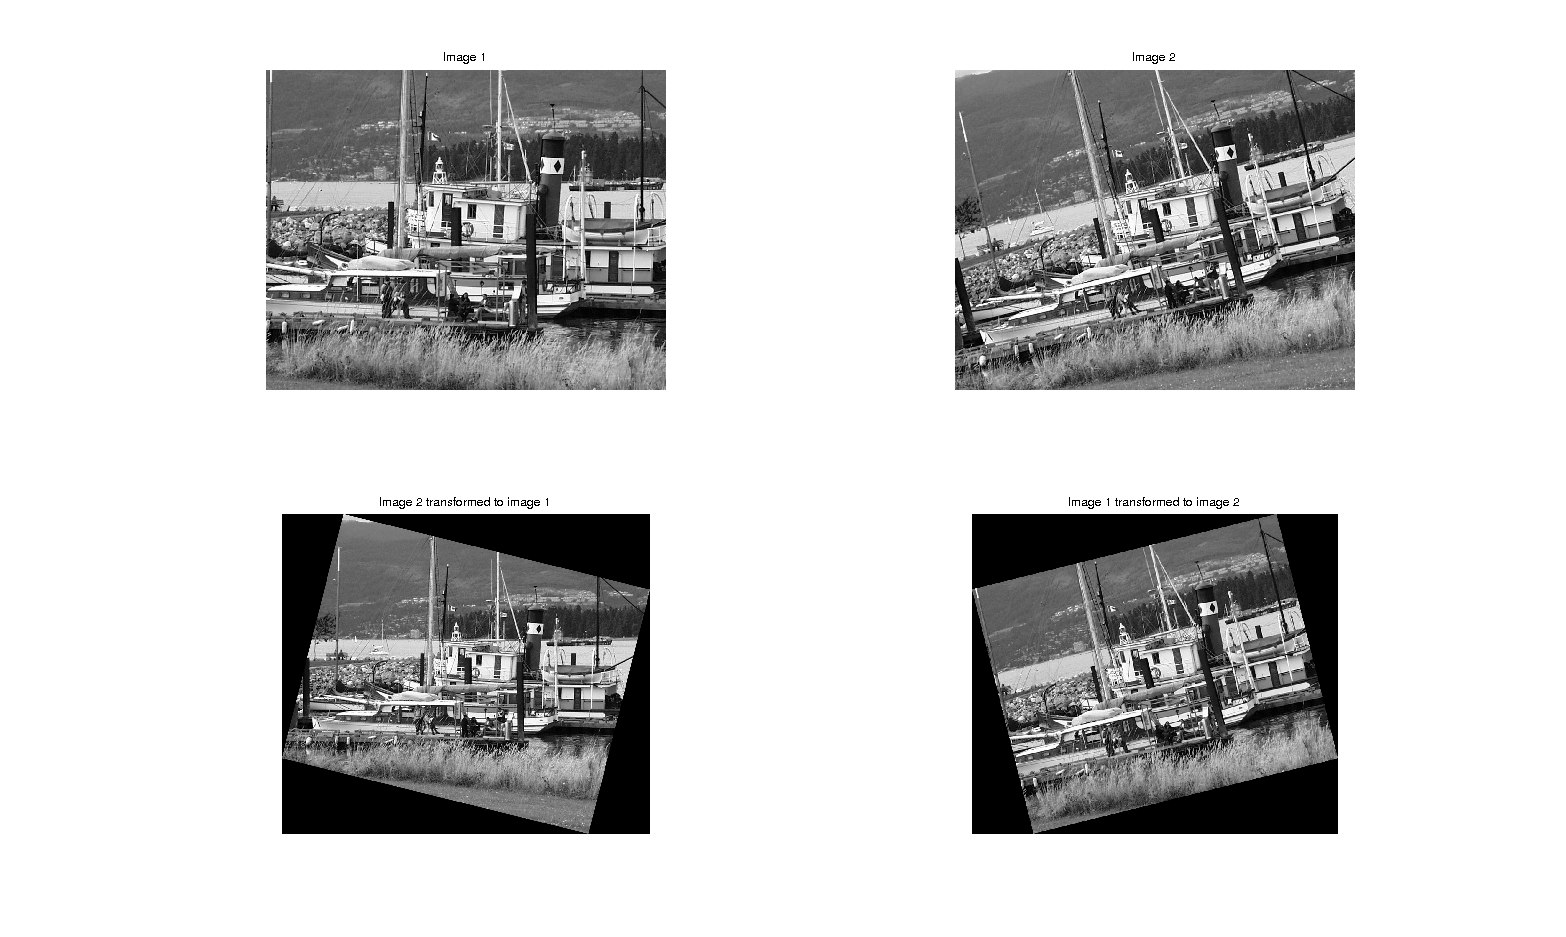
\includegraphics[width=1\textwidth]{img/transformedimg}
\caption{Affine transformation of the left image to the right image, and vice versa.}
\label{fig:transformedA}
\end{figure}

\subsection{The number of RANSAC iterations}
In our basic RANSAC implementation, convergence is usually very fast.
For the tram image, we found through informal investigation, that only about 8 out of 67 point correspondences appear to be outliers.
This means that the probability of picking three inliers is $(59/67)^3 \approx 0.68$.
For this reason, the algorithm often finds the correct transformation in the first few iterations on this image.

There is an easy way to estimate the number of iterations that have to be performed to be reasonably sure to have found the true transformation.
Let $q$ be the probability of sampling three inliers, and no outliers.
If we perform $h$ iterations, the probability that all $h$ seed samples will be `contaminated' (i.e. contain one or more outliers) is given by $(1-q)^h$.
We want to choose $h$ so that this quantity is below some acceptable level: $(1-q)^h \leq \epsilon$.
If we invert this inequality, we find
\begin{equation}
h \geq \left( \frac{\log \epsilon}{\log{1-q}} \right)
\end{equation}

However, since we do not know $q$, we cannot use this relation directly.
The probability of sampling a set of $k=3$ inliers can be expressed in terms of the number of matches $N$ and the number of inliers $N_I$:
\begin{equation}
q = \frac{\binom{N_I}{k}}{\binom{N}{k}} \approx \left(\frac{N_I}{N}\right)^k.
\label{eq:q}
\end{equation}

where the approximate equality holds when $N_I,N \gg k$ (which will almost certainly hold for our case $k=3$.
We still cannot use this formula directly because we do not know $N_I$.
However, the number of inliers of the current best model is a conservative estimate of $N_I$, so we can use it instead of $N_I$ in equation \ref{eq:q}.
We have implemented this method to determine the number of iterations $h$, see \verb+ransacA.m+.

As mentioned, under the present conditions the RANSAC algorithm usually converges in one iteration.
This is good, but does not bring out the richness in the operation of RANSAC, nor does it show the usefulness of our analytic choice of $h$.
To see more of the behaviour of RANSAC, we can decrease the accuracy of the found matches by decreasing the threshold that SIFT uses for rejecting matches based on the distance-ratio.
In figure \ref{fig:inliercount}, we have plotted two graphs where the inlier count of the best model is plotted against the iteration.
We see clearly that when the threshold has a good value, RANSAC quickly finds the right transformation, after which the inlier count remains stable (i.e. the algorithm has converged).
On the other hand, when more false matches are found due to a bad threshold setting, RANSAC takes a while to sample a good triple of points, but once it does, the estimated transformation is the same, and so is the inlier count (59).

\begin{figure}

        \centering
        \begin{subfigure}[b]{0.475\textwidth}
                \centering
                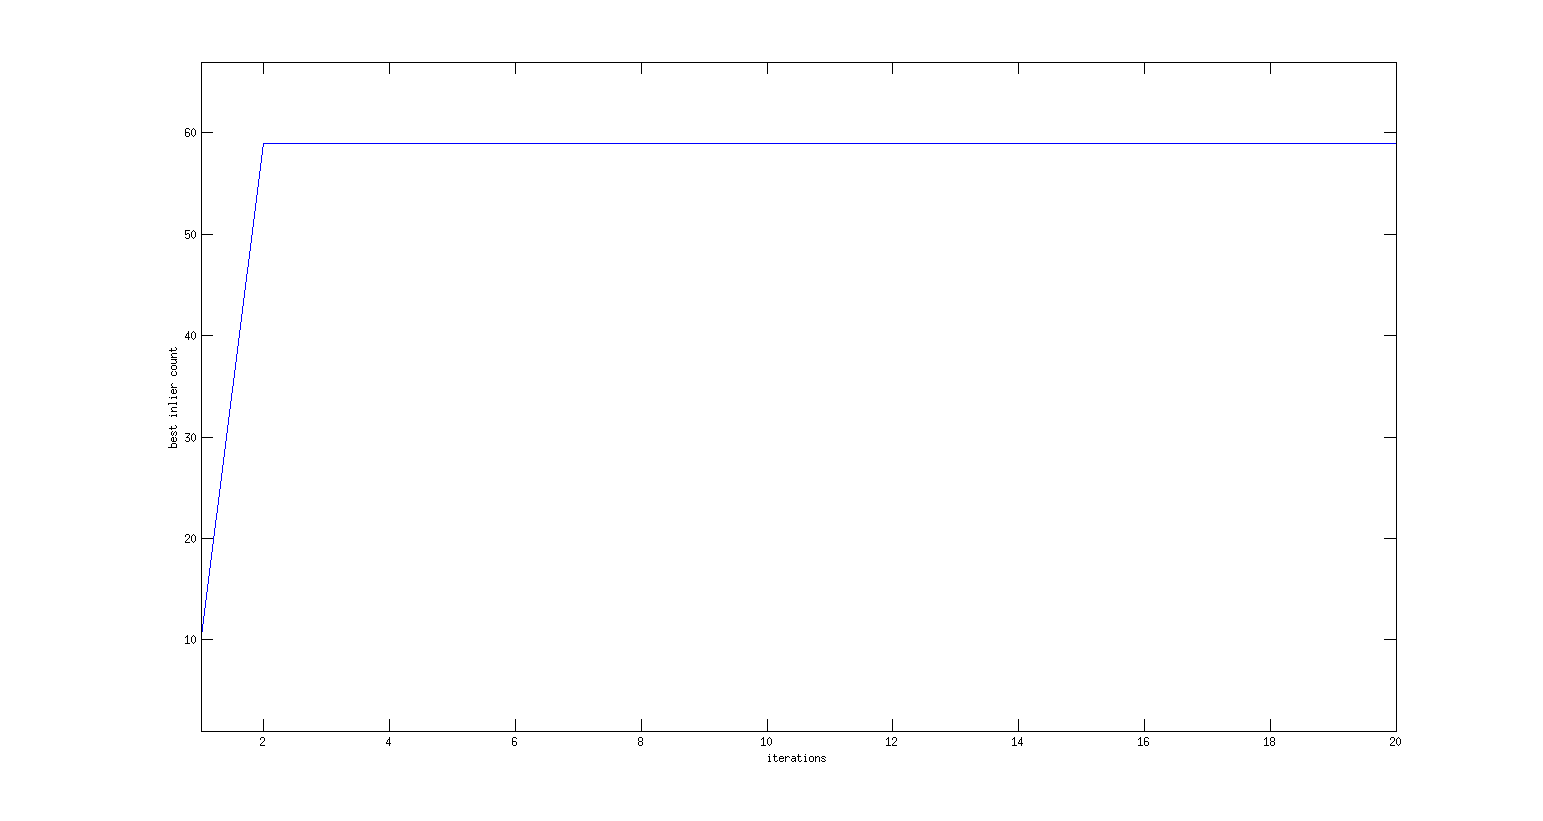
\includegraphics[width=\textwidth]{img/inliercount}
                \caption{Inlier count versus iteration for normal parameter settings (Standard SIFT distance ratio threshold).}
        \end{subfigure}
        ~
        \begin{subfigure}[b]{0.475\textwidth}
                \centering
                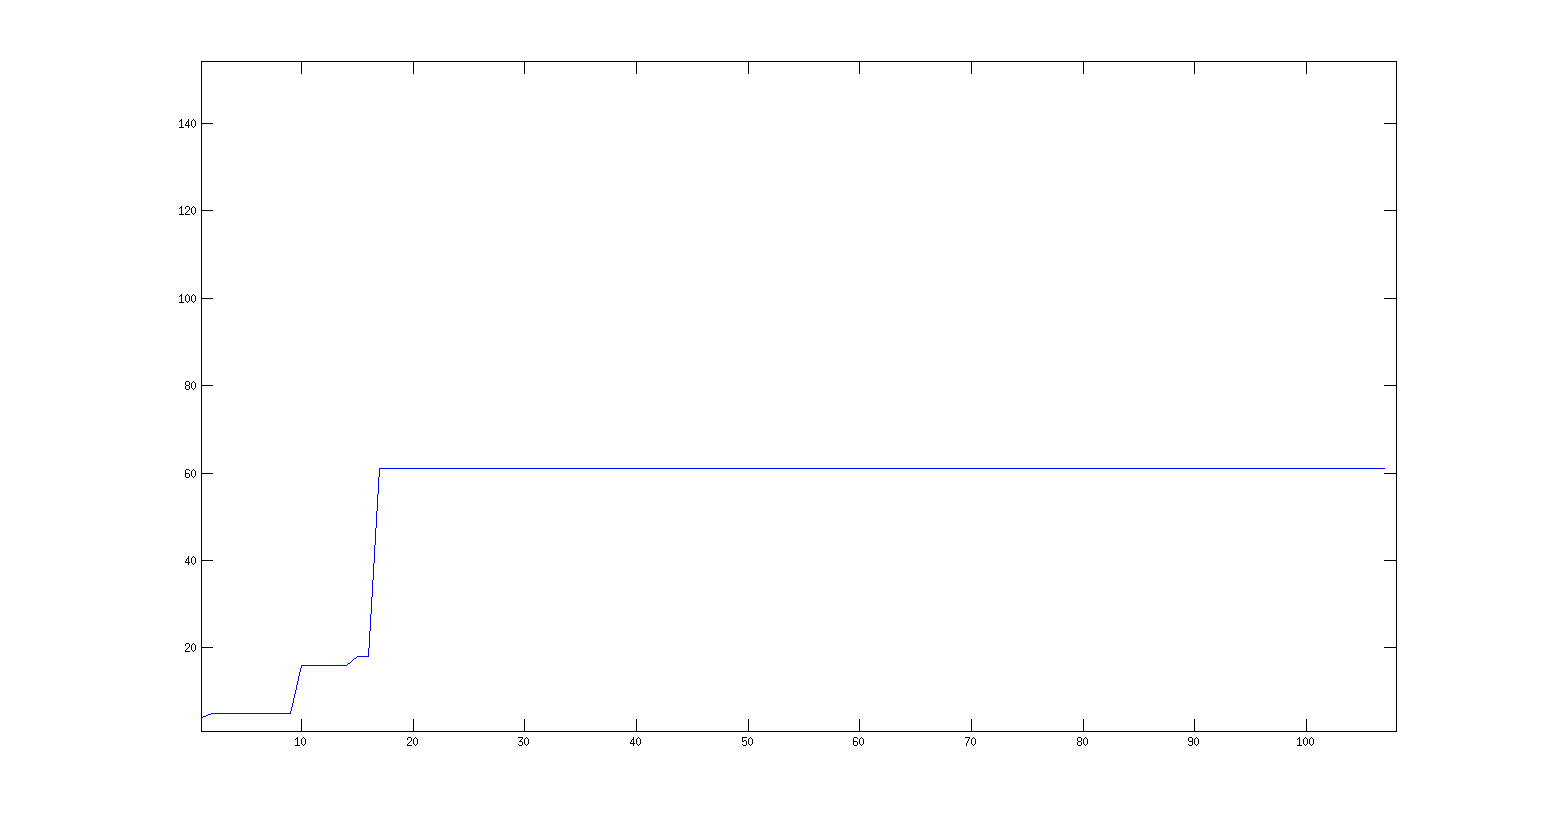
\includegraphics[width=\textwidth]{img/inliercount_11}
                \caption{Inlier count versus iteration for high-noise condition (low SIFT distance ratio threshold).}
        \end{subfigure}
\caption{Best model inlier count over multiple iterations with low and high noise setting}
\label{fig:inliercount}      
\end{figure}

\section{Image Stitching}
We can use the estimated affine transformation to stitch a series of images.
This is done by estimating the Affine transformation as in the previous section, and then using it to transform several images to one target image.
To do this, we repeatedly estimate the transformation from the current frame to the previous one, and transform each image to the first frame by the product of all transforms found so far.

We can either overlay each frame over the previous one, or use some method to combine pixel values for which we have measurements in multiple source images.
We opt for the latter approach, using matlab's \verb+nanmean+, \verb+nanmedian+, \verb+nanmin+ or \verb+nanmax+.
This allows us to use the mean/median/min/max function without being affected by black borders around the image.

To see the stitching in action, run \verb+StitchingDemo.m+.
This script loads the images and calls \verb+mosaic.m+, which takes a list of images and produces a stitched result.
This function is mainly concerned with the determination of the size of the final image, and with transforming each image with a transformation matrix.
The matching is done in \verb+imageAlign.m+, which calls the \verb+vl_feat+ functions and \verb+ransacA.m+.

The results can be seen in figure \ref{fig:affinestitch}.

\begin{figure}
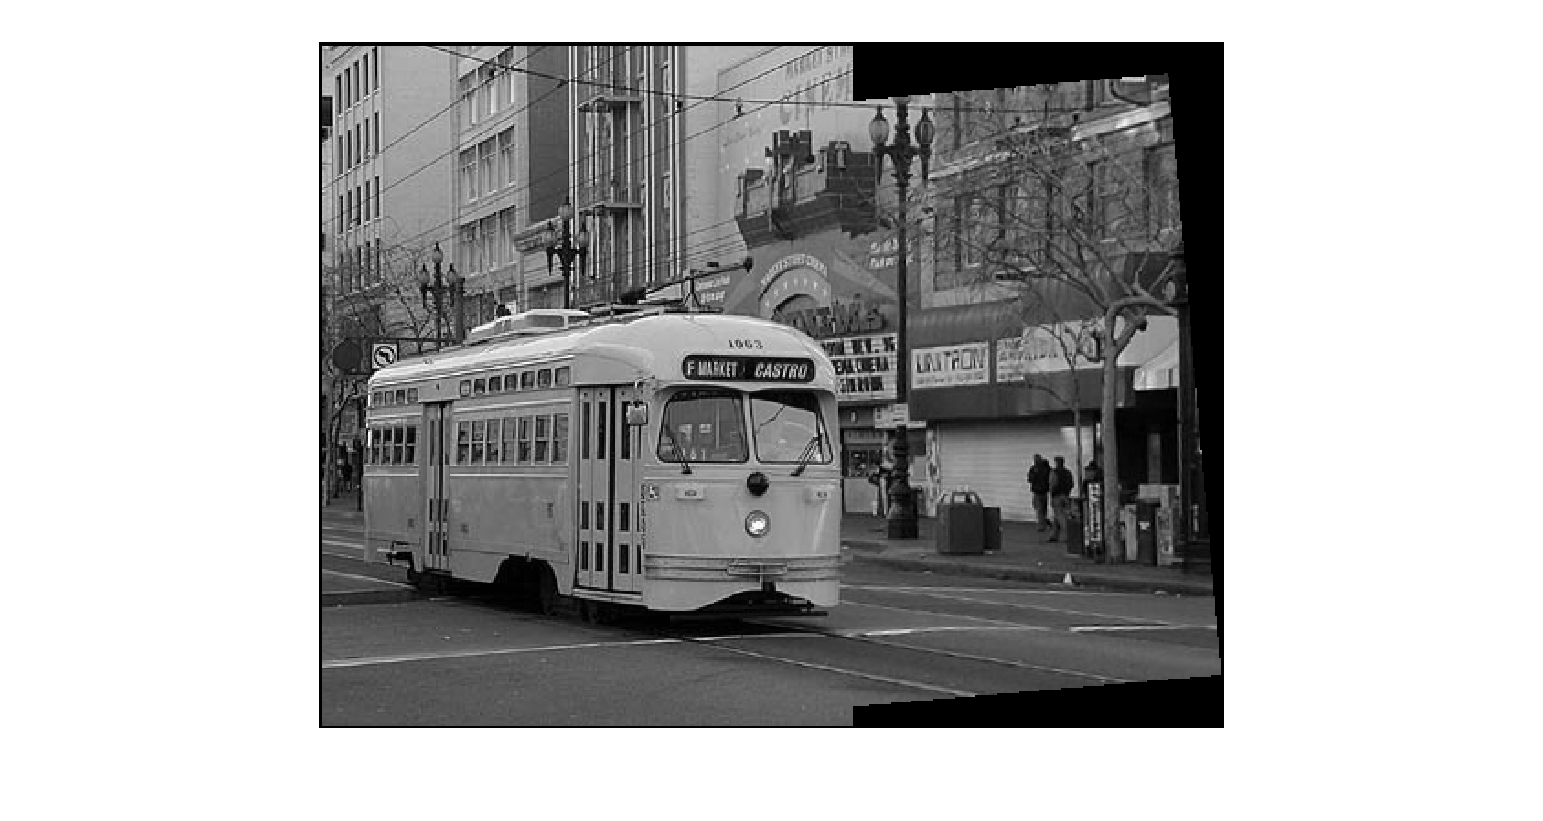
\includegraphics[width=1\textwidth]{img/affinestitch}
\caption{The result of stitching using an affine transformation.}
\label{fig:affinestitch}
\end{figure}

\section{Homography}
As a bonus, we implemented homography estimation and used it to stitch two images, as in the previous assignment.
The process is similar to the affine case, but this time we opted to solve using the SVD (for no particular reason).
We construct a matrix $A$ containing the homogeneous equations of the system.
Let $M$ be the projective matrix we want to estimate, then we want to have $M\mathbf{x} = \mathbf{x'} = (\lambda x', \lambda y', \lambda)^T$ for a point $\mathbf{x}$ and corresponding point $\mathbf{x'}$.
We can rearange to put the entries of $M$ in a vector $\mathbf{m}$, and put the elements of $\mathbf{x}$ and $\mathbf{x'}$ in $A$ so that they multiply the right elements of $\mathbf{m}$.
Since the rows of $A$ correspond to homogeneous equations (i.e. equations with a zero at the right-hand side), we will want to minimize $A\mathbf{m}$.
As stated, we use SVD for this; if $A = U S V$, then the least squares solution to $A\mathbf{m} = 0$ will be the last column of $V$.

To run the homography demo, run \verb+HomographyDemo.m+ or \verb+HomographyColorDemo.m+.
The result is shown in figure \ref{fig:stitchedhomo}.

\begin{figure}
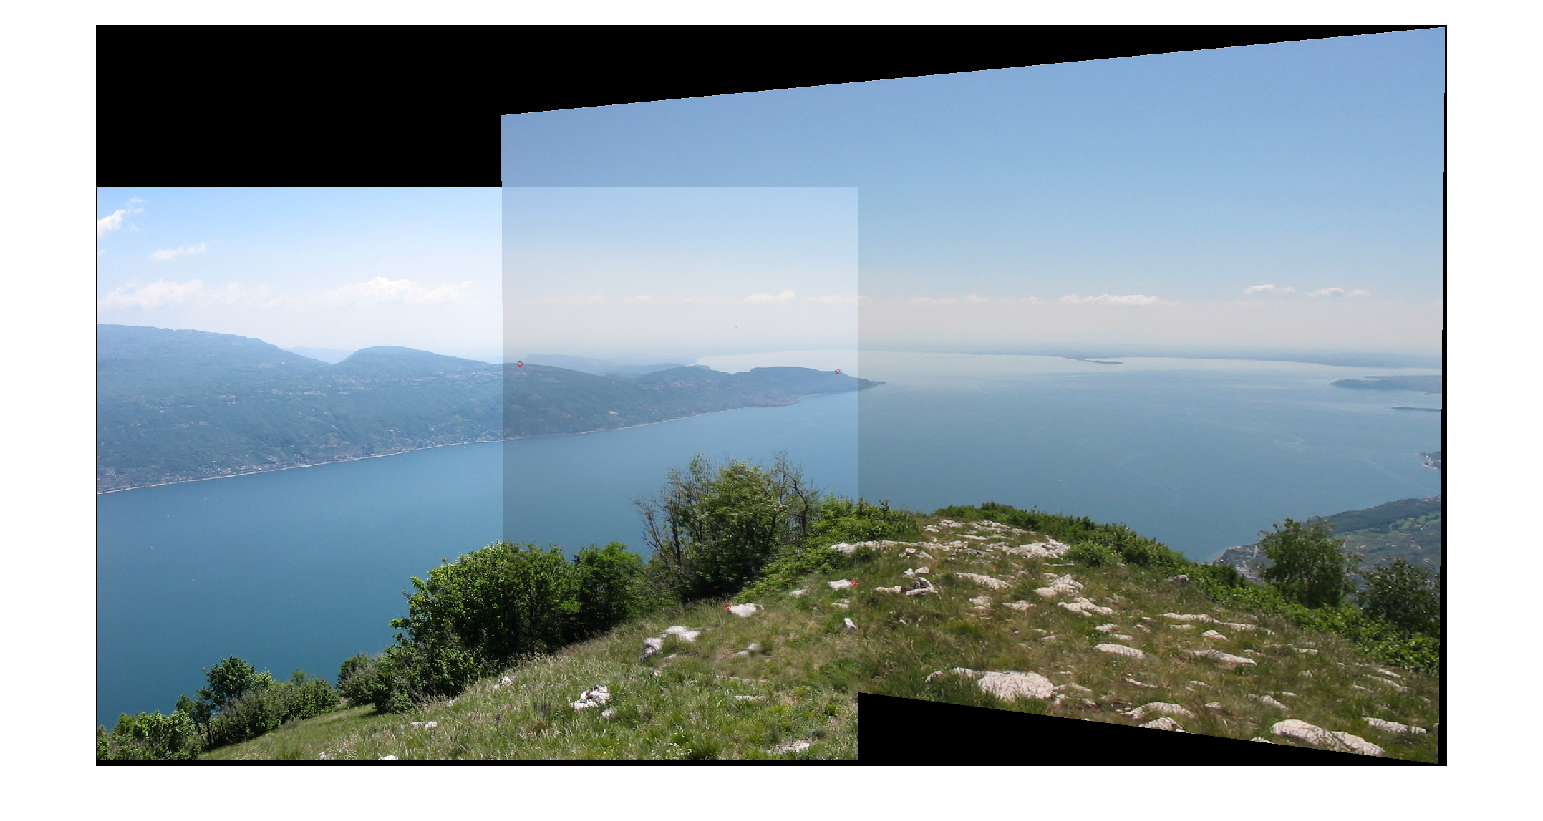
\includegraphics[width=1\textwidth]{img/homographycolorstitch2}
\caption{The result of stitching using a projective transformation. The transformation clearly does not preserve parallelism as in the case of affine transformations, because the transformed image is not a parallelogram. It does preserve colinearity.}
\label{fig:stitchedhomo}
\end{figure}

\end{document}
